\documentclass{standalone}
\usepackage{tikz}
\usepackage{ctex,siunitx}
\usepackage{tkz-euclide}
\usepackage{amsmath}
\usetikzlibrary{patterns, calc}
\usetikzlibrary {decorations.pathmorphing, decorations.pathreplacing, decorations.shapes,}
\begin{document}
\small
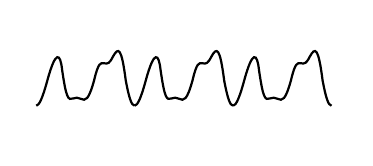
\begin{tikzpicture}[>=stealth, scale=0.5]
  \useasboundingbox(-0.5,1.34)rectangle(7.55,-1.47);
  \foreach \x in {0,2.5,5}
  {
    \begin{scope}[xshift=\x cm]
    \draw[thick]
    (-0.282,-0.642)..controls(-0.206,-0.638)and(-0.119,-0.436)..
( 0.000, 0.000)..controls( 0.215, 0.789)and( 0.329, 0.697)..
( 0.376, 0.261)..controls( 0.477,-0.429)and( 0.523,-0.518)..
( 0.656,-0.458)..controls( 0.707,-0.433)and( 0.788,-0.429)..
( 0.843,-0.465)..controls( 0.973,-0.531)and( 1.047,-0.500)..
( 1.187, 0.000)..controls( 1.294, 0.458)and( 1.355, 0.452)..
( 1.437, 0.436)..controls( 1.542, 0.416)and( 1.577, 0.433)..
( 1.664, 0.601)..controls( 1.806, 0.861)and( 1.883, 0.840)..
( 1.991, 0.000)..controls( 2.069,-0.418)and( 2.137,-0.646)..( 2.218,-0.642);
    \end{scope}
  }
\end{tikzpicture}
\end{document}